
%(BEGIN_QUESTION)
% Copyright 2006, Tony R. Kuphaldt, released under the Creative Commons Attribution License (v 1.0)
% This means you may do almost anything with this work of mine, so long as you give me proper credit

Studer det hydrauliske skjemadiagrammet for et reverserende sylindersystem:

$$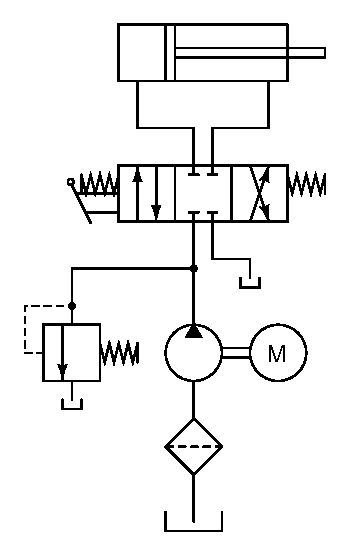
\includegraphics[width=15.5cm]{i00754x01.eps}$$

Når hendelen trekkes, beveger sylinderstempelet seg i én retning. Når hendelen skyves, beveger det seg i motsatt retning. Når hendelen slippes, fjærreturnerer den til midtstilling, og stempelet blir stående der det er.

\vskip 10pt

Identifiser hver komponent i systemet, og forklar i detalj hvordan systemet fungerer i hver av reguleringsventilens tre posisjoner. Vurder også om stempelet er låst i posisjon eller flytende når den retningsstyrte spoolventilen står i midtstilling.

\vskip 20pt \vbox{\hrule \hbox{\strut \vrule{} {\bf Forslag til sokratisk diskusjon} \vrule} \hrule}

\begin{itemize}
\item{} En kritisk viktig ferdighet ved tolkning av fluidkraftdiagrammer er å kunne avgjøre hva en spoolventil gjør når aktuatoren (håndtak, solenoidespole osv.) aktiveres. Forklar med egne ord hvordan du visualiserer «boks»-symbologien i praksis.
\item{} Anta at denne hydraulikksylinderen driver løftemekanismen på en gaffeltruck, og du legger merke til at løftet sakte siger ned mot bakken når motoren på trucken er slått av. Forklar hvorfor et hydraulisk løft kan sige ned, og angi konkret hva som skjer i hydraulikkskjemaet.
\item{} Kan dette stempelet yte samme kraft i begge retninger, eller er det sterkere i én retning enn den andre? Forklar dette i detalj.
\end{itemize}

\underbar{file i00754}
%(END_QUESTION)





%(BEGIN_ANSWER)


%(END_ANSWER)





%(BEGIN_NOTES)

Når hendelen skyves, beveger stempelet seg mot høyre. Når hendelen trekkes, beveger stempelet seg mot venstre. Stempelet låses i posisjon når spoolventilen står i midten, fordi begge linjene til sylinderen da er stengt, og hydraulikkolje er inkompressibel.

\filbreak \vskip 20pt \vbox{\hrule \hbox{\strut \vrule{} {\bf Virtuell feilsøking} \vrule} \hrule}

\noindent
{\bf Forutsi effekt av en gitt feil:} presenter hver av følgende feil for studentene, én om gangen, og la dem beskrive alle effektene feilen kan gi.

\begin{itemize}
\item{} Hydraulikkoljefilter tetter seg
\item{} Trykkregulator tetter seg
\item{} Linjen på venstre side av stempelaktuatoren får lekkasje
\item{} Nedoverpil-banens strømningsvei i spoolventilen tetter seg
\item{} Trykkregulator feiler helt åpen
\item{} Lekkasje oppstår mellom filter og pumpe
\end{itemize}

\vskip 10pt

\noindent
{\bf Identifiser mulige/umulige feil:} anta at sylinderen ikke beveger seg i noen retning når ventilen flyttes til noen av stillingene. Et manometer koblet til utløpet fra hydraulikkpumpen viser 1200 PSI, som er normalt. Vurder om følgende foreslåtte feil kan forklare alle symptomene, og forklar {\it hvorfor} eller {\it hvorfor ikke} for hver feil:

\begin{itemize}
\item{} Trykkregulator feilet helt åpen
\item{} Trykkregulator feilet stengt (tettet)
\item{} Hydraulikkoljefilter tett
\item{} Luftbobler i hydraulikkoljen
\item{} Reservoirport på spoolventilen tett
\item{} Elektromotor går for sakte
\item{} Venstre sylinderlinje tett
\item{} Høyre sylinderlinje tett
\end{itemize}

\vskip 10pt

\noindent
{\bf Vurder nytte av gitte diagnostiske tester:} tenk deg at ??? feiler ??? i dette systemet (men ikke fortell dette til studentene!). Presenter operatørens observasjoner, la studentene vurdere mulige feil og diagnosemetoder, og foreslå deretter følgende diagnostiske tester én etter én. La studentene vurdere verdien av hver test, dvs. om testen gir nyttig informasjon (forteller noe vi ikke allerede vet).

\begin{itemize}
\item{} {\it }
\item{}  -- {\bf Ja/Nei}
\item{}  -- {\bf Ja/Nei}
\end{itemize}

\vskip 10pt

\noindent
{\bf Diagnostiser en feil basert på gitte symptomer:} tenk deg at ??? feiler ??? i dette systemet (men ikke fortell dette til studentene!). Presenter operatørens observasjoner, la studentene tenke gjennom mulige feil og diagnosemetoder, og gi deretter resultatene av testene de foreslår ut fra symptomene, helt til de har identifisert feiltype og feilsted korrekt.

\begin{itemize}
\item{} {\it }
\item{}
\item{}
\end{itemize}

%INDEX% Mekanikk, fluidkraftsystemer: reverserende styring av dobbeltvirkende sylinder

%(END_NOTES)


